\documentclass[twoside]{book}

\usepackage[paperwidth=148mm, paperheight=210mm]{geometry}
\usepackage{fontspec}
%\usepackage[latin1]{inputenc}
\usepackage[nolocalmarks]{polyglossia}
\setdefaultlanguage[variant=french, frenchitemlabels=false]{french}
\usepackage[strict]{changepage}
\usepackage{fancyhdr}
\usepackage{paracol}
\usepackage{tableof}
\usepackage{setspace}
\usepackage{alltt}
\usepackage{titlesec}
\usepackage{xcolor}
\usepackage{xstring}
\usepackage{enumitem}

%%%%%%%%%%%%%%%%%%%%%%%%%%%%%%%%%%%%%%%%%%%%%%%%%%% Mise ne page %%%%%%%%%%%%%%%%%%%%%%%%%%%%%%
% on numérote les nbp par page et non globalement
\usepackage[perpage]{footmisc}

% définition des en-têtes et pieds de page
\pagestyle{empty}
\fancyhead{}
\fancyfoot{}
\renewcommand{\headrulewidth}{0pt}
\setlength{\headheight}{10pt}
\fancyhead[RO]{\small\thepage}
\fancyhead[LE]{\small\thepage}
% la commande titres permet de changer les titres de gauche et de droite.
\newcommand{\titres}[2]{
	\renewcommand{\rightmark}{\textcolor{red}{\sc #2}}
	\renewcommand{\leftmark}{\textcolor{red}{\sc #1}}
}
\titres{}{}

% pas d'indentation
\setlength{\parindent}{0mm}

\geometry{
inner=25mm,
outer=12mm,
top=15mm,
bottom=15mm,
headsep=3mm,
}

%%%%%%%%%%%%%%%%%%%%%%%%%%%%%%%%%%%%%%%%%%%%%%%%% Options gregorio %%%%%%%%%%%%%%%%%%%%%%%%%

\usepackage[forcecompile]{gregoriotex}
%\usepackage{gregoriotex}

%% style général de gregorio :
% lignes rouges, commenter pour du noir
%\gresetlinecolor{gregoriocolor}

% texte <alt> (au-dessus de la portée) en rouge et en petit, avec réglage de sa position verticale
\grechangestyle{abovelinestext}{\color{gregoriocolor}\footnotesize}
\newcommand{\altraise}{0 mm}
\grechangedim{abovelinestextraise}{\altraise}{scalable}

% taille des initiales
\newcommand{\initialsize}[1]{
    \grechangestyle{initial}{\fontspec{Zallman Caps}\fontsize{#1}{#1}\selectfont}
}
\newcommand{\defaultinitialsize}{28}
\initialsize{\defaultinitialsize}
% espace avant et après les initiales
\newcommand{\initialspace}[1]{
  \grechangedim{afterinitialshift}{#1}{scalable}
  \grechangedim{beforeinitialshift}{#1}{scalable}
}
\newcommand{\defaultinitialspace}{0cm}
\initialspace{\defaultinitialspace}

%% sélection de la police de neumes
\gresetnabcfont{gresgmodern}{12} 

% on définit le système qui capture des headers pour générer des annotations
% cette commande sera appelée pour définir des abréviations ou autres substitutions
\newcommand{\resultat}{}
\newcommand{\abbrev}[3]{
  \IfSubStr{#1}{#2}{ \renewcommand{\resultat}{#3} }{}
}
\newcommand{\officepartannotation}[1]{
  \renewcommand{\resultat}{#1}
  \abbrev{#1}{ntro}{ {Intr.} }
  \abbrev{#1}{espo}{Resp.}
  \abbrev{#1}{ll}{All.}
  \abbrev{#1}{act}{Tract.}
  \abbrev{#1}{equen}{Seq.}
  \abbrev{#1}{ffert}{Off.}
  \abbrev{#1}{ommun}{Co.}
  \abbrev{#1}{ntip}{Ant.}
  \abbrev{#1}{ntic}{Cant.}
  \abbrev{#1}{Toni Communes}{}
  \abbrev{#1}{yrial}{}
  \greannotation{\resultat}
}
\newcommand{\modeannotation}[1]{
  \renewcommand{\resultat}{#1}
  \abbrev{#1}{1}{ {\sc i} }
  \abbrev{#1}{2}{ {\sc ii} }
  \abbrev{#1}{3}{ {\sc iii} }
  \abbrev{#1}{4}{ {\sc iv} }
  \abbrev{#1}{5}{ {\sc v} }
  \abbrev{#1}{6}{ {\sc vi} }
  \abbrev{#1}{7}{ {\sc vii} }
  \abbrev{#1}{8}{ {\sc viii} }
  \greannotation{\resultat}
}
\gresetheadercapture{office-part}{officepartannotation}{}
\gresetheadercapture{mode}{modeannotation}{string}

%%%%%%%%%%%%%%%%%%%%%%%%%%%%%%%%%%%%%%%%%%%%%% Graphisme %%%%%%%%%%%%%%%%%%%%%%%%%%%
% on définit l'échelle générale

\newcommand{\echelle}{0.85}

% on centre les titres et on ne les numérote pas
\titleformat{\section}[block]{\Large\filcenter\sc}{}{}{}
\titleformat{\subsection}[block]{\large\filcenter\sc}{}{}{}
\titleformat{\paragraph}[block]{\filcenter\sc}{}{}{}
\setcounter{secnumdepth}{0}
% on diminue l'espace avant les titres
\titlespacing*{\paragraph}{0pt}{1ex}{.6ex}

% commandes versets, repons et croix
\newcommand{\vv}{\textcolor{red}{\fontspec[Scale=\echelle]{Charis SIL}℣.\hspace{3mm}}}
\newcommand{\rr}{\textcolor{red}{\fontspec[Scale=\echelle]{Charis SIL}℟.\hspace{3mm}}}
\newcommand{\cc}{\textcolor{red}{\fontspec[Scale=\echelle]{FreeSerif}\symbol{"2720}~}}
\renewcommand{\aa}{\textcolor{red}{\fontspec[Scale=\echelle]{Charis SIL}\Abar.\hspace{3mm}}}
\gresetspecial{V/}{\textcolor{gregoriocolor}{\fontspec{Charis SIL}℣.~}}
\gresetspecial{R/}{\textcolor{gregoriocolor}{\fontspec{Charis SIL}℟.~}}
\gresetspecial{A/}{\textcolor{gregoriocolor}{\fontspec{Charis SIL}\Abar.~}}
\gresetspecial{+}{{\fontspec{FreeSerif}†~}}
\gresetspecial{*}{\gresixstar}
\gresetspecial{cross}{\textcolor{gregoriocolor}{\fontspec{FreeSerif}\symbol{"2720}}}
\gresetspecial{labiacross}{\textcolor{gregoriocolor}{+}}

% commandes diverses
\newcommand{\antiphona}{\textcolor{red}{\noindent Antiphona.\hspace{4mm}}}
\newcommand{\antienne}{\textcolor{red}{\noindent Antienne.\hspace{4mm}}}
\newcommand{\rubrique}[1]{\textcolor{red}{\emph{#1}}}
\newcommand{\saut}{\hspace{1cm}}
\newcommand{\minisaut}{\hspace{4mm}}
\newcommand{\sautRV}{\\ \null \hspace{5.95mm}}
\newcommand{\petitvspace}{\vspace{2mm}}
\newcommand{\microvspace}{\vspace{0.8mm}}
% pour affichier 1 en rouge et un peu d'espace
\newcommand{\un}{{\color{gregoriocolor} 1~~~}}

% abréviations
\newcommand{\tpalleluia}{\rubrique{(T.P.} \mbox{Allelúia.\rubrique{)}}}
\newcommand{\tpalleluiafr}{\rubrique{(T.P.} \mbox{Alléluia.\rubrique{)}}}

\newcommand{\tqomittitur}{{\small \rubrique{(In Tempore Quadragesimæ ommittitur} Allelúia.\rubrique{)}}}
\newcommand{\careme}{{\small \rubrique{(Pendant le Carême on omet l'}Alléluia.\rubrique{)}}}

% environnement hymne : alltt + normalfont + marges custom
\newenvironment{hymne}
  {
  \begin{adjustwidth}{1.6cm}{1mm}
  \begin{alltt}\normalfont
  }
  {
  \end{alltt}
  \end{adjustwidth}
  }
  
% la commande \u permet de souligner les inflexions
\let\u\underline

% on définit la police par défaut
\setmainfont[Ligatures=TeX, Scale=\echelle]{Charis SIL}
%renderer=ICU a l'air de ne plus marcher...
%\setmainfont[Renderer=ICU, Ligatures=TeX, Scale=\echelle]{Charis SIL}
\setstretch{0.9}

% paramétrage de paracol en mode 2 colonnes par page : taille des colonnes, séparateur
\columnratio{0.5}
\setlength{\columnsep}{1.5em}
\setlength{\columnseprule}{0.3pt}

\begin{document}

% ceci est pour conserver une numérotation ordinaire malgré paracol
\twosided[pb]

\begin{titlepage}
\centering\null

\vspace{1cm}

{\scshape\LARGE In Ascensione Domini}

\vspace{2cm}

{\scshape\Large Ad Matutinum}

\vspace{5cm}

{\scshape\LARGE Ascension du Seigneur}

\vspace{2cm}

{\scshape\Large À Matines}


\end{titlepage}

% tolérance infinie sur les sauts de lignes pour les colonnes étroites
\sloppy
\gresetinitiallines{0}
\gregorioscore{partitions/ORIa}
\gresetinitiallines{1}
\emph{\vv Seigneur, ouvre mes lèvres. \minisaut \rr Et ma bouche annoncera ta louange. \\
\vv Dieu, viens à mon aide. \minisaut \rr Seigneur, viens vite à mon secours. \\
\vv Gloire au Père, au Fils, et au Saint-Esprit. \minisaut \rr Comme il était au commencement, maintenant et toujours, et dans les siècles des siècles. Amen. Alléluia.}

\section{Invitatoire}

\emph{\aa Alléluia, le Christ Seigneur qui monte au ciel, * Venez, adorons-le, alléluia.}

\gregorioscore{partitions/P5F5I_marteo}

\vfill

\emph{Venez, chantons avec allégresse au Seigneur, faisons monter l'expression d'une joie vers Dieu, notre salut.
Hâtons-nous de nous présenter devant lui avec des louanges et, dans des psaumes célébrons sa gloire.\\
Parce que le Seigneur est le grand Dieu; le grand Roi au dessus de tous les dieux; parce que le Seigneur ne repoussera pas son peuple; parce que dans sa main sont tous les confins de la terre et que son regard domine les cimes des montagnes.\\
Parce qu'à lui est la mer, et que c'est lui-même qui l'a faite, et que ses mains ont formé le continent. Venez, adorons, prosternons-nous devant Dieu, et pleurons devant le Seigneur qui nous a faits, parce que lui-même est le Seigneur notre Dieu, et que nous sommes son peuple et les brebis de son pâturage.\\
Aujourd'hui, si vous entendez sa voix, n'endurcissez pas vos cœurs, comme il arriva à vos pères dans l'exaspération au jour de la tentation dans le désert, alors qu'ils me tentèrent, m'éprouvèrent et virent mes œuvres.\\
Pendant quarante ans, j'ai été proche de cette génération et j'ai dit: Toujours ils errent de cœur; et eux, ils n'ont point connu mes voies: et je leur ai juré dans ma colère, s'ils entreront dans mon repos.}


\section{Hymne}
\gregorioscore{partitions/P5F5H_marteo}

~

\begin{paracol}{2}
\begin{alltt}\normalfont        Roi éternel et très haut,
        Rédempteur des fidèles,
        à qui la mort détruite a donné
        le triomphe de la gloire souveraine.

        Vous montez au-dessus des astres,
        où vous appelait la puissance
        sur toutes les choses,
        Puissance céleste et non humaine :

        Pour que le triple monde créé,
        du ciel, de la terre et des enfers,
        désormais soumis à votre empire,
        fléchissent le genou devant votre majesté.

        Les Anges tremblent en voyant
        renversé le sort des mortels :
        la chair pèche, la chair purifie,
        un Dieu règne dans la chair d’un Dieu.\end{alltt}

\switchcolumn
\begin{alltt}\normalfont    Soyez vous-même notre joie,
    demeurant au ciel notre récompense,
    vous qui gouvernez l’univers créé,
    triomphant des joies du monde.

    D’ici-bas, nous vous demandons instamment,
    pardonnez toutes les offenses,
    élevez vers vous les cœurs,
    par la vertu de la céleste grâce.

    Afin qu’au moment où, soudain, vous commencerez
    à briller sur la nuée du juge
    vous écartiez de nous les châtiments mérités,
    vous rendiez les couronnes perdues.

    O Jésus, à Vous soit la gloire,
    Qui rentrez en vainqueur au ciel,
    Ainsi qu’au Père et à l’Esprit Saint,
    Dans les siècles éternels.\end{alltt}
\end{paracol}


\section{Premier nocturne}

\subsection{Psaume 8}

\gregorioscore{partitions/P5F5N1A1_marteo}
\aa \emph{O Dieu, votre magnificence * s’est élevée au-dessus des cieux, alléluia.}

\gresetinitiallines{0}
\gregorioscore{partitions/ps8_4e}
\gresetinitiallines{1}

\un \emph{Seigneur, notre Maître, * que Votre Nom est admirable dans toute la terre !}
\begin{paracol}{2}
\begin{enumerate}[wide, itemsep=0mm, labelwidth=!, labelindent=0pt, label=\color{gregoriocolor}\theenumi]
\setcounter{enumi}{1}
TODO
\end{enumerate}
\switchcolumn
\begin{enumerate}[wide, itemsep=0mm, labelwidth=!, labelindent=0pt, before=\itshape, label=\color{gregoriocolor}\theenumi]
\setcounter{enumi}{1}
\item Car Votre magnificence est élevée * au-dessus des cieux.
\item De la bouche des enfants et de ceux qui sont à la mamelle Vous avez tiré une louange parfaite contre Vos adversaires, * pour détruire l'ennemi, et celui qui veut se venger.
\item Quand je considère Vos cieux, qui sont l'ouvrage de Vos doigts, * la lune et les étoiles que Vous avez créées,
\item Je m'écrie : Qu'est-ce que l'homme, pour que Vous Vous souveniez de lui ? * ou le fils de l'homme, pour que Vous le visitiez ?
\item Vous ne l'avez mis qu'un peu au-dessous des Anges ; Vous l'avez couronné de gloire et d'honneur, * et Vous l'avez établi sur les ouvrages de Vos mains.
\item Vous avez mis toutes choses sous ses pieds, * toutes les brebis, et tous les bœufs, et même les animaux des champs,
\item Les oiseaux du ciel, et les poissons de la mer, * qui parcourent les sentiers de l'océan.
\item Seigneur, notre Maître, * que Votre Nom est admirable dans toute la terre !
\end{enumerate}
\end{paracol}

\subsection{Psaume 10}

\gregorioscore{partitions/P5F5N1A2_marteo}
\aa \emph{Le Seigneur est dans son saint temple, le Seigneur est dans le ciel, alléluia.}

\gresetinitiallines{0}
\gregorioscore{partitions/ps10_8}
\gresetinitiallines{1}

\un \emph{Je me confie au Seigneur ; comment dites-vous à mon âme : * Emigrez sur la montagne comme un passereau ?}
\begin{paracol}{2}
\begin{enumerate}[wide, itemsep=0mm, labelwidth=!, labelindent=0pt, label=\color{gregoriocolor}\theenumi]
\setcounter{enumi}{1}
TODO
\end{enumerate}
\switchcolumn
\begin{enumerate}[wide, itemsep=0mm, labelwidth=!, labelindent=0pt, before=\itshape, label=\color{gregoriocolor}\theenumi]
\setcounter{enumi}{1}
\item Car voici que les pécheurs ont tendu leur arc ; ils ont préparé leurs flèches dans leur carquois, * pour tirer dans l'ombre contre ceux qui ont le cœur droit.
\item Car ce que vous aviez établi, ils l'ont détruit ; * mais le juste, qu'a-t-il fait ?
\item Le Seigneur est dans Son saint temple ; * le Seigneur a Son trône dans le Ciel.
\item Ses yeux regardent le pauvre ; * Ses paupières examinent les enfants des hommes.
\item Le Seigneur examine le juste et l'impie ; * or celui qui aime l'iniquité hait son âme.
\item Il fera pleuvoir des pièges sur les pécheurs ; * le feu, et le soufre, et le vent des tempêtes, sont la part de leur calice.
\item Car le Seigneur est juste, et Il aime la justice ; * Son visage contemple l'équité.
\end{enumerate}
\end{paracol}

\subsection{Psaume 18}

\gregorioscore{partitions/P5F5N1A3_marteo}
\aa \emph{Du plus haut du ciel part sa course, qui s’achève en ce même sommet, alléluia.}

\gresetinitiallines{0}
\gregorioscore{partitions/ps18_4e}
\gresetinitiallines{1}

\un \emph{Les cieux racontent la gloire de Dieu, * et le firmament publie les œuvres de Ses mains.}
\begin{paracol}{2}
\begin{enumerate}[wide, itemsep=0mm, labelwidth=!, labelindent=0pt, label=\color{gregoriocolor}\theenumi]
\setcounter{enumi}{1}
TODO
\end{enumerate}
\switchcolumn
\begin{enumerate}[wide, itemsep=0mm, labelwidth=!, labelindent=0pt, before=\itshape, label=\color{gregoriocolor}\theenumi]
\setcounter{enumi}{1}
\item Le jour proclame ce message au jour, * et la nuit en donne connaissance à la nuit.
\item Ce ne sont point des paroles, ce n'est pas un langage * dont la voix ne soit pas entendue.
\item Leur bruit s'est répandu dans toute la terre, * et leurs accents jusqu'aux extrémités du monde.
\item Il a établi Sa tente dans le soleil, * qui est lui-même semblable à un époux sortant de sa chambre nuptiale.
\item Il s'est élancé comme un géant pour fournir sa carrière. * Il sort de l'extrémité du ciel,
\item Et sa course va jusqu'à l'autre extrémité, * et il n'y a personne qui se dérobe à sa chaleur.
\item La loi du Seigneur est sans tache, elle restaure les âmes ; * le témoignage du Seigneur est fidèle, il donne la sagesse aux petits.
\item Les justices du Seigneur sont droites, elles réjouissent les cœurs ; * le précepte du Seigneur est lumineux, il éclaire les yeux.
\item La crainte du Seigneur est sainte, elle subsiste à jamais ; * les jugements du Seigneur sont vrais, ils se justifient par eux-mêmes.
\item Ils sont plus désirables que l'or et que beaucoup de pierres précieuses ; * ils sont plus doux que le miel, et qu'un rayon plein de miel.
\item Aussi Votre serviteur les observe ; * à les garder, on trouve une grande récompense.
\item Qui connaît ses fautes ? Purifiez-moi de celles qui sont cachées en moi, * et préservez Votre serviteur de la corruption des étrangers.
\item S'ils ne me dominent point, alors je serai sans tache, * et purifié d'un très grand péché.
\item Et alors les paroles de ma bouche pourront Vous plaire, * et la méditation de mon cœur sera toujours en Votre présence.
\item Seigneur, Vous êtes mon secours * et mon rédempteur.
\end{enumerate}
\end{paracol}

\subsection{Versicule}
\begin{paracol}{2}
\vv Ascéndit Deus in jubilatióne, allelúia. \\
\rr Et Dóminus in voce tubæ, allelúia. \\
\vv Pater noster... \rubrique{(secrètement)} Et ne nos indúcas in tentatiónem. \\
\rr Sed líbera nos a malo. \\
\vv Exáudi, Dómine Iesu Christe, preces servórum tuórum, \GreSpecial{+} et mise\textit{rére} \textbf{no}bis: * Qui cum Patre et Spíritu Sancto vivis et regnas in sǽcula sæculórum. \rr Amen.
\switchcolumn
\vv Dieu s’est élevé au milieu des acclamations, alléluia. \\
\rr Et le Seigneur au son de la trompette, alléluia. \\
\vv Notre Père... Et ne nous laissez pas succomber à la tentation. \\
\rr Mais délivrez-nous du mal. \\
\vv Exaucez, Seigneur Jésus-Christ, les prières de vos serviteurs, et ayez pitié de nous, vous qui vivez et régnez avec le Père et le Saint-Esprit, dans les siècles des siècles. \rr Amen.
\end{paracol}


\subsection{Première leçon}

\begin{paracol}{2}
\vv Jube, domne, benedícere. \\
\vv Benedictió\textit{ne} \textit{per}\textbf{pé}tua benedícat nos Pater ætérnus.\\
\rr Amen.\\
\switchcolumn
\vv Veuillez, Seigneur, bénir. \\
\vv Que le Père éternel nous bénisse d'une bénédiction perpétuelle. \\
\rr Amen.
\end{paracol}

\paragraph{Commencement du Livre des Aces des Apôtres.} \rubrique{Ac 1: 1-5}

\begin{alltt}\normalfont{}Cher Théophile, dans mon premier livre,
	j’ai parlé de tout ce que Jésus a fait et enseigné,
	depuis le moment où il commença,
	jusqu’au jour où il fut enlevé au ciel, après avoir, par l’Esprit Saint,
	donné ses instructions aux Apôtres qu’il avait choisis.
C’est à eux qu’il s’est présenté vivant après sa Passion;
	il leur en a donné bien des preuves, puisque, pendant quarante jours,
	il leur est apparu et leur a parlé du royaume de Dieu.
Au cours d’un repas qu’il prenait avec eux,
	il leur donna l’ordre de ne pas quitter Jérusalem,
	mais d’y attendre que s’accomplisse la promesse du Père.
Il déclara: «Cette promesse, vous l’avez entendue de ma bouche:
	alors que Jean a baptisé avec l’eau,
	vous, c’est dans l’Esprit Saint que vous serez baptisés d’ici peu de jours.»\end{alltt}
\begin{paracol}{2}
\vv Tu autem, Dómine, miserére nobis. \\
\rr Deo grátias.
\switchcolumn
\vv Et vous Seigneur, ayez pitié de nous. \\
\rr Rendons grâces à Dieu.
\end{paracol}

\vfill

\gregorioscore{partitions/P5F5N1R1_marteo}

\emph{\rr Après sa passion, pendant quarante jours, il leur apparaissait et leur parlait du royaume de Dieu, alléluia :
* Puis, devant leurs yeux, il s’éleva, alléluia : et une nuée le déroba à leurs regards, alléluia.
\vv Et mangeant avec eux, il leur ordonna de ne pas s’éloigner de Jérusalem, mais d’attendre ce qu’avait promis le Père.}

\subsection{Deuxième leçon}

\begin{paracol}{2}
\vv Jube, domne, benedícere. \\
\vv Unigénitus \textit{Dei} \textbf{Fí}lius * nos benedícere et adjuváre dignétur.\\
\rr Amen.
\switchcolumn
\vv Veuillez, Seigneur, bénir. \\
\vv Que le Fils unique de Dieu daigne nous bénir et nous secourir.\\
\rr Amen.
\end{paracol}

\rubrique{Ac 1: 6-9}

\begin{alltt}\normalfont{}Ainsi réunis, les Apôtres l’interrogeaient:
	«Seigneur, est-ce maintenant le temps où tu vas rétablir le royaume pour Israël?»
Jésus leur répondit: «Il ne vous appartient pas de connaître
		les temps et les moments que le Père a fixés de sa propre autorité.
Mais vous allez recevoir une force quand le Saint-Esprit viendra sur vous;
	vous serez alors mes témoins à Jérusalem,
	dans toute la Judée et la Samarie, et jusqu’aux extrémités de la terre.»
Après ces paroles, tandis que les Apôtres le regardaient,
	il s’éleva, et une nuée vint le soustraire à leurs yeux.\end{alltt}

\begin{paracol}{2}
\vv Tu autem, Dómine, miserére nobis. \\
\rr Deo grátias.
\switchcolumn
\vv Et vous Seigneur, ayez pitié de nous. \\
\rr Rendons grâces à Dieu.
\end{paracol}

\vfill

\gregorioscore{partitions/P5F5N1R2_marteo}

\emph{\rr Toute la beauté du Seigneur a été exaltée au-dessus des astres :
* Son rayonnement est dans les nuées du ciel, et son nom demeure éternellement, alléluia. \\
\vv Du plus haut du ciel part sa course, qui s'achève en ce même sommet.}

~

\subsection{Troisième leçon}

~

\begin{paracol}{2}
\vv Jube, domne, benedícere. \\
\vv Spíritus \text{Sancti} \textbf{grá}tia illúminet sensus et corda nostra.\\
\rr Amen.
\switchcolumn
\vv Veuillez, Seigneur, bénir. \\
\vv Que la grâce du Saint-Esprit illumine nos esprits et nos cœurs.\\
\rr Amen.
\end{paracol}

\rubrique{Ac 1: 10-14}

\begin{alltt}\normalfont{}Et comme ils fixaient encore le ciel où Jésus s’en allait,
	voici que, devant eux, se tenaient deux hommes en vêtements blancs,
	qui leur dirent: «Galiléens, pourquoi restez-vous là à regarder vers le ciel?
	Ce Jésus qui a été enlevé au ciel d’auprès de vous,
	viendra de la même manière que vous l’avez vu s’en aller vers le ciel.»
Alors, ils retournèrent à Jérusalem
		depuis le lieu-dit «mont des Oliviers» qui en est proche,
	la distance de marche ne dépasse pas ce qui est permis le jour du sabbat.
À leur arrivée,
	ils montèrent dans la chambre haute où ils se tenaient habituellement;
	c’était Pierre, Jean, Jacques et André, Philippe et Thomas, Barthélemy et Matthieu,
	Jacques fils d’Alphée, Simon le Zélote, et Jude fils de Jacques.
Tous, d’un même cœur, étaient assidus à la prière,
	avec des femmes, avec Marie la mère de Jésus, et avec ses frères.\end{alltt}


\begin{paracol}{2}
\vv Tu autem, Dómine, miserére nobis. \\
\rr Deo grátias.
\switchcolumn
\vv Et vous Seigneur, ayez pitié de nous. \\
\rr Rendons grâces à Dieu.
\end{paracol}

\gregorioscore{partitions/P5F5N1R3_marteo}

\emph{\rr Élevez-vous, Seigneur, alléluia,
* Dans votre force, alléluia,
\vv Votre magnificence s’est élevée au-dessus des cieux.}

\section{Deuxième nocturne}

\subsection{Psaume 20}

\gregorioscore{partitions/P5F5N2A1_marteo}
\aa \emph{Élevez-vous, Seigneur, dans votre force : nous voulons chanter et psalmodier, alléluia.}

\gresetinitiallines{0}
\gregorioscore{partitions/ps20_4e}
\gresetinitiallines{1}
\un \emph{Seigneur, le roi se réjouira dans Votre force, * et il tressaillira d'une vive allégresse, parce que Vous l'aurez sauvé.}
\begin{paracol}{2}

\begin{enumerate}[wide, itemsep=0mm, labelwidth=!, labelindent=0pt, label=\color{gregoriocolor}\theenumi]
\setcounter{enumi}{1}
TODO
\end{enumerate}

\switchcolumn
\begin{enumerate}[wide, itemsep=0mm, labelwidth=!, labelindent=0pt, before=\itshape, label=\color{gregoriocolor}\theenumi]
\setcounter{enumi}{1}
\item Vous lui avez accordé le désir de son cœur, * et Vous ne l'avez point frustré de la demande de ses lèvres.
\item Car Vous l'avez prévenu des plus douces bénédictions ; * Vous avez mis sur sa tête une couronne de pierres précieuses.
\item Il vous a demandé la vie, * et Vous lui avez accordé des jours qui dureront dans les siècles des siècles.
\item Sa gloire est grande, grâce à Votre salut ; * Vous le couvrirez de gloire et d'un honneur immense.
\item Car Vous ferez de lui une source de bénédictions perpétuelles ; * Vous le comblerez de joie en lui montrant Votre visage.
\item Car le roi espère au Seigneur, * et la miséricorde du Très-Haut le rendra inébranlable.
\item Que votre main atteigne tous Vos ennemis ; * que votre droite trouve tous ceux qui vous haïssent.
\item Vous en ferez comme une fournaise ardente, au temps où vous montrerez votre visage irrité ; * le Seigneur dans Sa colère les remplira de trouble, et le feu les dévorera.
\item Vous exterminerez leur fruit de dessus la terre, * et leur race d'entre les enfants des hommes.
\item Car ils ont fait tomber des maux sur vous ; * ils ont formé des desseins qu'ils n'ont pu exécuter.
\item Car vous leur ferez tourner le dos ; * vous préparerez leur visage à recevoir les traits qui vous restent.
\item Levez-Vous, Seigneur, dans Votre force ; * nous chanterons et nous célébrerons Vos actions d'éclat.
\end{enumerate}

\end{paracol}

\subsection{Psaume 29}

\gregorioscore{partitions/P5F5N2A2_marteo}
\aa \emph{Je vous exalterai, Seigneur, parce que vous m’avez accueilli, alléluia.}

\gresetinitiallines{0}
\gregorioscore{partitions/ps29_8}
\gresetinitiallines{1}

\un \emph{Je Vous exalterai, Seigneur, parce que Vous m'avez relevé, * et que Vous n'avez pas réjoui mes ennemis à mon sujet.}
\begin{paracol}{2}
\begin{enumerate}[wide, itemsep=0mm, labelwidth=!, labelindent=0pt, label=\color{gregoriocolor}\theenumi]
\setcounter{enumi}{1}
TODO
\end{enumerate}
\switchcolumn
\begin{enumerate}[wide, itemsep=0mm, labelwidth=!, labelindent=0pt, before=\itshape, label=\color{gregoriocolor}\theenumi]
\setcounter{enumi}{1}
\item Seigneur mon Dieu, j'ai crié vers Vous, * et Vous m'avez guéri.
\item Seigneur, Vous avez retiré mon âme du séjour des morts ; * Vous m'avez sauvé du milieu de ceux qui descendent dans la fosse.
\item Chantez au Seigneur, Vous qui êtes Ses saints, * et célébrez Sa sainte mémoire.
\item Car le châtiment provient de Son indignation, * et la vie de Sa bienveillance.
\item Les pleurs se répandent le soir, * et le matin viendra la joie.
\item Pour moi j'ai dit dans ma prospérité : * Je ne serai jamais ébranlé.
\item Seigneur, c'est par Votre volonté * que Vous m'avez affermi dans ma gloire.
\item Vous avez détourné de moi Votre visage, * et j'ai été tout troublé.
\item Je crierai vers Vous, Seigneur, * et j'implorerai mon Dieu.
\item Quelle utilité retirerez-Vous de ma mort, * lorsque je descendrai dans la pourriture ?
\item Est-ce que la poussière chantera Vos louanges ? * ou publiera-t-elle Votre vérité ?
\item Le Seigneur a entendu, et Il a eu pitié de moi ; * le Seigneur S'est fait mon protecteur.
\item Vous avez changé mes lamentations en allégresse ; * Vous avez déchiré mon sac, et Vous m'avez environné de joie,
\item Afin que mon âme Vous chante, et que je ne ressente plus la douleur. * Seigneur mon Dieu, je Vous louerai éternellement.
\end{enumerate}
\end{paracol}

\subsection{Psaume 46}

\gregorioscore{partitions/P5F5N2A3_marteo}
\aa \emph{Dieu s’est élevé au milieu des acclamations, et le Seigneur au son de la trompette, alléluia.}

\gresetinitiallines{0}
\gregorioscore{partitions/ps46_4e}
\gresetinitiallines{1}

\un \emph{Nations, frappez toutes des mains ; * célébrez Dieu par des cris d'allégresse.}
\begin{paracol}{2}

\begin{enumerate}[wide, itemsep=0mm, labelwidth=!, labelindent=0pt, label=\color{gregoriocolor}\theenumi]
\setcounter{enumi}{1}
TODO
\end{enumerate}

\switchcolumn
\begin{enumerate}[wide, itemsep=0mm, labelwidth=!, labelindent=0pt, before=\itshape, label=\color{gregoriocolor}\theenumi]
\setcounter{enumi}{1}
\item Car le Seigneur est très haut et terrible, * Roi suprême sur toute la terre.
\item Il nous a assujetti les peuples, * et a mis les nations sous nos pieds.
\item Il nous a choisis pour Son héritage ; * la beauté de Jacob qu'Il a aimée.
\item Dieu est monté au milieu des cris de joie, * et le Seigneur au son de la trompette.
\item Chantez à notre Dieu, chantez ; * chantez à notre Roi, chantez.
\item Car Dieu est le Roi de toute la terre ; * chantez avec sagesse.
\item Dieu régnera sur les nations ; * Dieu est assis sur Son saint trône.
\item Les princes des peuples se sont unis au Dieu d'Abraham ; * car les dieux puissants de la terre ont été extraordinairement élevés.
\end{enumerate}

\end{paracol}

\subsection{Versicule}
\begin{paracol}{2}
\vv Ascéndens Christus in altum, allelúia. \\
\rr Captívam duxit captivitátem, allelúia. \\
\vv Pater noster... \rubrique{(secrètement)} Et ne nos indúcas in tentatiónem. \\
\rr Sed líbera nos a malo. \\
\vv Ipsíus píetas et misericórdi\textit{a} \textit{nos} \textbf{ád}juvet, * qui cum Patre et Spíritu Sancto vivit et regnat in sǽcula sæculórum. \\
\rr Amen.
\switchcolumn
\vv Le Christ montant au ciel, alléluia. \\
\rr A emmené captive la captivité, alléluia. \\
\vv Notre Père... Et ne nous laissez pas succomber à la tentation. \\
\rr Mais délivrez-nous du mal. \\
\vv Qu'il nous secoure par sa bonté et sa miséricorde, celui qui, avec le Père et le Saint-Esprit, vit et règne dans les siècles des siècles. \rr Amen.
\end{paracol}


\subsection{Quatrième leçon}

\begin{paracol}{2}
\vv Jube, domne, benedícere. \\
\vv Deus Pa\textit{ter om}\textbf{ní}potens * sit nobis propítius et clemens. \\
\rr Amen.
\switchcolumn
\vv Veuillez, Seigneur, bénir. \\
\vv Que Dieu le Père tout-puissant soit pour nous propice et plein de clémence. \\
\rr Amen.
\end{paracol}

\paragraph{Sermon de saint Léon Pape.}
Depuis la bienheureuse et glorieuse résurrection de Notre Seigneur Jésus-Christ, dans laquelle le vrai temple de Dieu, détruit par l'impiété juive, a été relevé en trois jours par la divine puissance, voici aujourd’hui, mes bien-aimés, le quarantième jour. Le nombre de ces saints jours s’est accompli en vertu d’une très sainte disposition, et a été employé utilement à notre instruction. L’intention du Seigneur, en prolongeant pendant ce temps sa présence corporelle, était de fortifier, par des preuves indubitables, la foi en sa résurrection. Car la mort du Christ avait beaucoup troublé les cœurs des disciples ; son supplice sur la croix, son dernier soupir, 1’ensevelissement de son cadavre avaient accablé leurs esprits d’une telle tristesse, qu’une certaine torpeur de défiance s’y était glissée.
\begin{paracol}{2}
\vv Tu autem, Dómine, miserére nobis. \\
\rr Deo grátias.
\switchcolumn
\vv Et vous Seigneur, ayez pitié de nous. \\
\rr Rendons grâces à Dieu.
\end{paracol}


\gregorioscore{partitions/P5F5N2R1_marteo}

\emph{\rr C’est le temps de m’en retourner à celui qui m’a envoyé, dit le Seigneur : ne vous attristez pas et que votre coeur ne soit pas troublé :
* Je prie pour vous le Père de vous garder lui-même, alléluia, alléluia. \\
\vv Si je ne m’en vais pas, le Paraclet ne viendra pas : c’est après mon ascension que je vous l'enverrai.}

\subsection{Cinquième leçon}

\begin{paracol}{2}
\vv Jube, domne, benedícere. \\
\vv Chris\texit{tus per}\textbf{pé}tuæ * det nobis gáudia vitæ.\\
\rr Amen.
\switchcolumn
\vv Veuillez, Seigneur, bénir. \\
\vv Que le Christ nous donne les joies de l'éternelle vie.\\
\rr Amen.
\end{paracol}
Et c’est ainsi que les bienheureux Apôtres et tous les disciples, d’abord effrayés de la mort sur la croix et fort hésitants dans leur foi à la résurrection, ont été à ce point affermis par l’évidence de la vérité qu’à la vue du Seigneur s’en allant dans les hauteurs du ciel, non seulement ils n’ont pas éprouvé de tristesse, mais ils ont même été remplis de joie. Et certes bien grand et ineffable était leur motif de se réjouir, qu and, en présence d’une sainte multitude, on voyait la nature humaine monter plus haut en dignité que toutes les créatures célestes, pour dépasser les ordres angéliques et s’éleverau-dessus des Archanges. Elle ne devait connaître de terme aux sublimités de son élévation qu’une fois reçuepar le Père éternel, assodée à sa gloire, sur le trône decelui dont elle partage la nature en qualité de Fils.
\begin{paracol}{2}
\vv Tu autem, Dómine, miserére nobis. \\
\rr Deo grátias.
\switchcolumn
\vv Et vous Seigneur, ayez pitié de nous. \\
\rr Rendons grâces à Dieu.
\end{paracol}

\gregorioscore{partitions/P5F5N2R2_marteo}

\emph{\rr Que votre coeur ne se trouble pas ; je vais au Père, et quand j’aurai été enlevé d’au milieu de vous, je vous enverrai, alléluia,
* L’Esprit de vérité, et votre coeur se réjouira, alléluia,
\vv Je prierai le Père et ilvous enverra un autre Paraclet.}

\subsection{Sixième leçon}

\begin{paracol}{2}
\vv Jube, domne, benedícere. \\
\vv Ignem su\texit{i a}\textbf{mó}ris * accéndat Deus in córdibus nostris. \\
\rr Amen.
\switchcolumn
\vv Veuillez, Seigneur, bénir. \\
\vv Que Dieu daigne allumer dans nos cœurs le feu de son amour.\\
\rr Amen.
\end{paracol}
Puisque l’Ascension du Christ est notre propre élévation et qu’il y a espoir pour le corps d’être appelé où l’a précédé la gloire de sa tête, tressaillons donc, mes bien-aimés, de dignes sentiments de joie, et réjouissons-nous dans de pieuses actions de grâces. Aujourd’hui nous ne sommes pas seulement confirmés dans la possession du Paradis, mais, en la personne du Christ, nous avons pénétré au plus haut des cieux. Nous avons obtenu, par l’ineffable grâce du Christ, des biens meilleurs que ceux que nous avions perdus par la jalousie du diable. En effet, ceux que le venimeux ennemi a chassés de la félidté de leur premier habitat, le Fils de Dieu se les est incorporés et les a placés à la droite du Père, avec lequel, étant Dieu, il vit et règne dans l’unité du Saint-Esprit, dans tous les siècles des siècles. Amen.
\begin{paracol}{2}
\vv Tu autem, Dómine, miserére nobis. \\
\rr Deo grátias.
\switchcolumn
\vv Et vous Seigneur, ayez pitié de nous. \\
\rr Rendons grâces à Dieu.
\end{paracol}

\gregorioscore{partitions/P5F5N2R3_marteo}

\emph{\rr Montant au ciel, le Christ a conduit captive la captivité,
* Il a donné des dons aux hommes, alléluia, alléluia, alléluia.
\vv Dieu s’est élevé au milieu des acclamations, et le Seigneur au son de la trompette.}

\section{Troisième nocturne}

\subsection{Psaume 96}

\gregorioscore{partitions/P5F5N3A1_marteo}
\aa \emph{Il a été infiniment élevé, alléluia : au-dessus de tous les dieux, alléluia.}

\gresetinitiallines{0}
\gregorioscore{partitions/ps96_6}
\gresetinitiallines{1}
\un \emph{Le Seigneur est Roi : que la terre tressaille de joie, * que toutes les îles se réjouissent.}
\begin{paracol}{2}

\begin{enumerate}[wide, itemsep=0mm, labelwidth=!, labelindent=0pt, label=\color{gregoriocolor}\theenumi]
\setcounter{enumi}{1}
TODO
\end{enumerate}
\switchcolumn
\begin{enumerate}[wide, itemsep=0mm, labelwidth=!, labelindent=0pt, before=\itshape, label=\color{gregoriocolor}\theenumi]
\setcounter{enumi}{1}
\item La nuée et l'obscurité sont autour de Lui ; * la justice et l'équité sont le soutien de Son trône.
\item Le feu marche devant Lui, * et embrase autour de Lui Ses ennemis.
\item Ses éclairs ont brillé sur le monde ; * la terre a vu, et a tremblé.
\item Les montagnes se sont fondues comme la cire à la face du Seigneur ; * à la face du Seigneur, toute la terre.
\item Les cieux ont proclamé Sa justice, * et tous les peuples ont vu Sa gloire.
\item Qu'ils soient confondus tous ceux qui adorent les images sculptées, * et qui se glorifient dans leurs idoles.
\item Adorez-Le, vous tous Ses Anges. * Sion a entendu et s'est réjouie,
\item Et les filles de Juda ont tressailli de joie, * à cause de Vos jugements, Seigneur.
\item Car Vous êtes le Seigneur Très-Haut sur toute la terre ; * Vous êtes infiniment élevé au-dessus de tous les dieux.
\item Vous qui aimez le Seigneur, haïssez le mal ; * le Seigneur garde les âmes de Ses saints; Il les délivrera de la main du pécheur.
\item La lumière s'est levée pour le juste, * et la joie pour ceux qui ont le cœur droit.
\item Réjouissez-vous, justes, dans le Seigneur, * et célébrez la mémoire de Sa sainteté.
\end{enumerate}

\end{paracol}

\subsection{Psaume 98}

\gregorioscore{partitions/P5F5N3A2_marteo}
\aa \emph{Le Seigneur est dans Sion, alléluia : grand et élevé, alléluia.}

\gresetinitiallines{0}
\gregorioscore{partitions/ps98_6}
\gresetinitiallines{1}

\un \emph{Le Seigneur règne : que les peuples s'irritent. * Il est assis sur les chérubins : que la terre soit ébranlée.}
\begin{paracol}{2}

\begin{enumerate}[wide, itemsep=0mm, labelwidth=!, labelindent=0pt, label=\color{gregoriocolor}\theenumi]
\setcounter{enumi}{1}
TODO
\end{enumerate}

\switchcolumn
\begin{enumerate}[wide, itemsep=0mm, labelwidth=!, labelindent=0pt, before=\itshape, label=\color{gregoriocolor}\theenumi]
\setcounter{enumi}{1}
\item Le Seigneur est grand dans Sion, * et Il est élevé au-dessus de tous les peuples.
\item Qu'on rende gloire à Votre grand Nom, car il est terrible et saint, * et l'honneur du roi est d'aimer la justice.
\item Vous avez marqué les directions à suivre ; * Vous avez exercé la justice et le jugement dans Jacob.
\item Exaltez le Seigneur notre Dieu, et adorez l'escabeau de Ses pieds, * car il est saint.
\item Moïse et Aaron étaient parmi Ses prêtres, * et Samuel parmi ceux qui invoquent Son Nom.
\item Ils invoquaient le Seigneur, et Il les exauçait ; * Il leur parlait dans la colonne de nuée.
\item Ils gardaient Ses ordonnances, * et le précepte qu'Il leur avait donné.
\item Seigneur notre Dieu, Vous les exauciez ; * ô Dieu, Vous leur avez été propice, et Vous punissiez toutes leurs fautes.
\item Exaltez le Seigneur notre Dieu, et adorez-Le sur Sa montagne sainte, * car le Seigneur notre Dieu est saint.
\end{enumerate}

\end{paracol}

\subsection{Psaume 102}

\gregorioscore{partitions/P5F5N3A3_marteo}
\aa \emph{Le Seigneur, dans le ciel, * alléluia, a dressé son trône, alléluia.}

\gresetinitiallines{0}
\gregorioscore{partitions/ps102_6}
\gresetinitiallines{1}

\un \emph{Mon âme, bénis le Seigneur, * et que tout ce qui est au dedans de moi bénisse Son saint Nom.}
\begin{paracol}{2}

\begin{enumerate}[wide, itemsep=0mm, labelwidth=!, labelindent=0pt, label=\color{gregoriocolor}\theenumi]
\setcounter{enumi}{1}

TODO

\end{enumerate}

\switchcolumn
\begin{enumerate}[wide, itemsep=0mm, labelwidth=!, labelindent=0pt, before=\itshape, label=\color{gregoriocolor}\theenumi]
\setcounter{enumi}{1}
\item Mon âme, bénis le Seigneur, * et n'oublie jamais tous Ses bienfaits.
\item C'est Lui qui pardonne toutes tes iniquités, * et qui guérit toutes tes maladies.
\item C'est Lui qui rachète ta vie de la mort, * qui te couronne de miséricorde et de grâces.
\item C'est Lui qui remplit tes désirs en te comblant de biens ; * ta jeunesse sera renouvelée comme celle de l'aigle.
\item Le Seigneur fait miséricorde, * et Il rend justice à tous ceux qui souffrent la violence.
\item Il a fait connaître Ses voies à Moïse, * et Ses volontés aux enfants d'Israël.
\item Le Seigneur est compatissant et miséricordieux, * patient et très miséricordieux.
\item Il ne S'irritera pas perpétuellement, * et ne menacera pas sans fin.
\item Il ne nous a pas traités selon nos péchés, * et Il ne nous a pas punis selon nos iniquités.
\item Car autant le Ciel est élevé au-dessus de la terre, * autant Il a affermi Sa miséricorde sur ceux qui Le craignent.
\item Autant l'orient est éloigné du couchant, * autant Il a éloigné de nous nos iniquités.
\item Comme un père a compassion de ses enfants, ainsi le Seigneur a compassion de ceux qui Le craignent. * Car Il sait de quoi nous sommes formés ;
\item Il S'est souvenu que nous ne sommes que poussière. * Les jours de l'homme passent comme l'herbe ; il fleurit comme la fleur des champs.
\item Qu'un souffle passe sur lui, et il n'est plus, * et le lieu qu'il occupait ne le reconnaît plus.
\item Mais la miséricorde du Seigneur s'étend de l'éternité à l'éternité * sur ceux qui Le craignent.
\item Et Sa justice se répand sur les enfants des enfants * de ceux qui gardent Son alliance,
\item Et qui se souviennent de Ses préceptes, * pour les accomplir.
\item Le Seigneur a préparé Son trône dans le Ciel, * et tout sera assujetti à Son empire.
\item Bénissez le Seigneur, vous tous, Ses Anges, * qui êtes puissants et forts ; qui exécutez Sa parole, pour obéir à la voix de Ses ordres.
\item Bénissez le Seigneur, vous toutes, Ses armées ; * vous, Ses ministres, qui faites Sa volonté.
\item Bénissez le Seigneur, vous toutes, Ses œuvres, * dans tous les lieux de Sa domination. Mon âme, bénis le Seigneur.
\end{enumerate}

\end{paracol}


\subsection{Versicule}
\begin{paracol}{2}
\vv Ascéndo ad Patrem meum, et Patrem vestrum, allelúia. \\
\rr Deum meum, et Deum vestrum, allelúia. \\
\vv Pater noster... \rubrique{(secrètement)} Et ne nos indúcas in tentatiónem. \\
\rr Sed líbera nos a malo. \\
\vv A vínculis peccatórum nostrórum absólvat nos omnípotens et miséricors Dóminus. \rr Amen.
\switchcolumn
\vv Je monte vers mon Père et votre Père, alléluia, \\
\rr Mon Dieu et votre Dieu, alléluia. \\
\vv Notre Père... Et ne nous laissez pas succomber à la tentation. \\
\rr Mais délivrez-nous du mal. \\
\vv Que le Dieu tout-puissant et miséricordieux daigne nous délivrer des liens de nos péchés. \rr Amen.
\end{paracol}


\subsection{Septième leçon}

\begin{paracol}{2}
\vv Jube, domne, benedícere. \\
\vv Evangé\textit{lica} \texbf{lé}ctio * sit nobis salus et protéctio.
\rr Amen.
\switchcolumn
\vv Veuillez, Seigneur, bénir. \\
\vv Que la lecture du saint Evangile nous soit salut et protection. 
\rr Amen.
\end{paracol}

\paragraph{Léctio sancti Evangélii secúndum Marcum} \rubrique{Mc 16: 14-20}

En ce temps-là, Jésus se manifesta aux Onze eux-mêmes pendant qu’ils étaient à table : il leur reprocha leur manque de foi et la dureté de leurs cœurs parce qu’ils n’avaient pas cru ceux qui l’avaient contemplé ressuscité.\\
Et réliqua.

\paragraph{Homilía sancti Gregórii Papæ}

Le retard que les disciples mirent à croire à la résurrection du Seigneur, n’a pas tant été leur faiblesse, qu’elle n’a été, pour ainsi dire, notre assurance future. La résurrection, en effet, à raison de leur doute, fut démontrée par beaucoup de preuves ; et, lorsque nous lisons ces faits dans l’Évangile, ne sommes-nous pas affermis par leur hésitation même ? L’histoire de Madeleine qui crut très vite, m’est moins utile que celle de Thomas qui douta longtemps. Car cet Apôtre en doutant, toucha les cicatrices du Sauveur, et enleva ainsi de notre cœur la plaie du doute.

\begin{paracol}{2}
\vv Tu autem, Dómine, miserére nobis. \\
\rr Deo grátias.
\switchcolumn
\vv Et vous Seigneur, ayez pitié de nous. \\
\rr Rendons grâces à Dieu.
\end{paracol}

\gregorioscore{partitions/P5F5N3R1_marteo}

\emph{\rr Je prierai mon Père, et il vous donnera un autre Paraclet,
* L’Esprit de vérité, pour qu’il demeure éternellement avec vous, alléluia.\\
\vv Car, si je ne m’en vais point, le Paraclet ne viendra pas à vous ; mais si je m’en vais, je vous l’enverrai.}

\subsection{Huitième leçon}

\begin{paracol}{2}
\vv Jube, domne, benedícere. \\
\vv Diví\textit{num au}\textbf{xí}lium * máneat semper nobíscum.
\rr Amen.
\switchcolumn
\vv Veuillez, Seigneur, bénir. \\
\vv Que le secours divin demeure toujours avec nous.
\rr Amen.
\end{paracol}
Pour faire pénétrer en nous la vérité de la Résurrection du Seigneur, il nous faut aussi remarquer ces paroles de saint Luc : « Mangeant avec eux, il leur commanda de ne pas s’éloigner de Jérusalem. » Et un peu plus loin : « Eux le voyant, il s’éleva, et une nuée le déroba à leurs yeux. » Notez ces paroles, remarquez ces mystères. Après avoir mangé avec eux, il s’éleva ; il mangea et il monta, afin de nous rendre manifeste par l’action d’absorber de la nourriture, la réalité de sa chair. Saint Marc rapporte que le Seigneur, avant de monter au ciel, reprocha à ses disciples la dureté de leur cœur et leur incrédulité. Que remarquer en cela, sinon que le Seigneur adressa des reproches à ses disciples au moment où il les quittait corporellement, afin que ces paroles, dites en se séparant d’eux, restassent plus profondément imprimées dans le cœur de ceux qui les entendaient ?
\begin{paracol}{2}
\vv Tu autem, Dómine, miserére nobis. \\
\rr Deo grátias.
\switchcolumn
\vv Et vous Seigneur, ayez pitié de nous. \\
\rr Rendons grâces à Dieu.
\end{paracol}

\gregorioscore{partitions/P5F5N3R2_marteo}

\emph{\rr Vous montez, Seigneur, sur une nuée :
* Vous marchez sur les ailes des vents, alléluia.
\vv Vous êtes revêtu de louange et d’honneur, enveloppé de lumière, comme d’un vêtement.}

\subsection{Neuvième leçon}

\begin{paracol}{2}
\vv Jube, domne, benedícere. \\
\vv Ad societátem cívium supernórum perdúcat nos Rex Angelórum.
\rr Amen.
\switchcolumn
\vv Veuillez, Seigneur, bénir. \\
\vv Que le Roi des Anges nous fasse parvenir à la société des citoyens célestes.
\rr Amen.
\end{paracol}

Écoutons ce que le Sauveur commande à ses disciples, après leur avoir reproché leur endurcissement : « Allez dans tout l’univers, et prêchez l’Évangile à toute créature. » Est-ce à dire, mes frères, que le saint Évangile dût être annoncé aux choses inanimées, ou aux animaux dépourvus de raison, et que ce soit à leur sujet que cette parole ait été dite aux disciples : « Prêchez à toute créature ? » Mais c’est l’homme qui est désigné ici par ces mots : toute créature. L’homme a, en effet, quelque chose de toute créature. L’être lui est commun avec les pierres, la vie avec les arbres, la sensibilité avec les animaux, et l’intelligence avec les Anges. Si donc l’homme a quelque chose de commun avec toute créature, on peut dire, en quelque sorte, que l’homme est toute créature, et par conséquent l’Évangile est prêché à toute créature, lorsqu’il est prêché à l’homme seul.

\begin{paracol}{2}
\vv Tu autem, Dómine, miserére nobis. \\
\rr Deo grátias.
\switchcolumn
\vv Et vous Seigneur, ayez pitié de nous. \\
\rr Rendons grâces à Dieu.
\end{paracol}


\section{Te Deum}
\gresetnabc{1}{invisible}
\gregorioscore{partitions/ORTDb_dcrochu}

~

\emph{{\footnotesize
Nous Vous louons ô Dieu: * nous Vous reconnaissons pour le Seigneur. \\
Ô Père éternel * toute la terre vous révère. \\
Tous les Anges * les Cieux, et toutes les Puissances, \\
Les Chérubins et les Séraphins * Vous proclament sans cesse: \\
Saint, Saint, Saint * le Seigneur, le Dieu des armées. \\
Les Cieux et la terre sont remplis * de la majesté de Votre gloire. \\
Le chœur glorieux * des Apôtres, \\
Le phalange vénérable * des Prophètes, \\
L'armée des Martyrs éclatante de blancheur * célèbre Vos louanges; \\
La sainte Eglise confesse * Votre nom par toute la terre, \\
Ô Père * d'infinie majesté! \\
Et elle vénère Votre Fils * véritable et unique. \\
Ainsi que le Saint-Esprit * consolateur. \\
Vous êtes le Roi de gloire * ô Christ! \\
Vus êtes du Père * le Fils éternel. \\
Pour délivrer l'homme * Vous n'avez pas eu horreur du sein d'une Vierge. \\
Vous avez brisé l'aiguillon de la mort * et ouvert aux fidèles le royaume des cieux. \\
Vous êtes assis à la droite de Dieu * dans la gloire du Père. \\
Nous croyons que vous êtes le juge * qui doit venir. \\
Nous Vous supplions donc de secourir vos serviteurs * que Vous avez rachetés par Votre Sang précieux. \\
Faites qu'ils soient au nombre des saints, * dans la gloire éternelle. \\
Sauvez Votre peuple, Seigneur * et bénissez Votre héritage. \\
Conduisez Vos serviteurs * et élevez-les jusque dans l'éternité. \\
Chaque jour * nous Vous bénissons. \\
Et nous louons Votre nom dans les siècles; * et dans les siècles des siècles. \\
Daignez Seigneur, en ce jour * nous préserver de tout péché. \\
Ayez pitié de nous Seigneur, * ayez pitié de nous. \\
Que Votre miséricorde, Seigneur se répande sur nous, * selon que nous avons éspéré en Vous. \\
J'ai éspéré en Vous Seigneur; * que je ne sois pas confondu à jamais.}}

~

\begin{paracol}{2}
\vv Dóminus vobíscum.\\
\rr Et cum spíritu tuo.
\switchcolumn
\vv Le Seigneur soit avec vous.\\
\rr Et avec votre esprit.
\switchcolumn*
\vv Orémus.\\
Concéde, quǽsumus, omnípotens Deus: ut, qui hodiérna die Unigénitum tuum, Redemptórem nostrum, ad cælos ascendísse crédimus; ipsi quoque mente in cæléstibus habitémus.
Per eúmdem Dóminum nostrum Jesum Christum Fílium tuum, qui tecum vivit et regnat in unitáte Spíritus Sancti, Deus, per ómnia sǽcula sæculórum. \rrrub Amen.
\switchcolumn
\vv Prions.  Accordez à notre prière, Dieu tout-puissant, puisque nous croyons qu’aujourd’hui Votre Fils unique, notre Rédempteur, est monté aux cieux, que nous habitions aussi en esprit au céleste séjour.
Par le même Jésus Christ, Votre Fils, notre Seigneur, Lui qui vit et règne avec Vous et le Saint-Esprit, Dieu, maintenant et pour les siècles des siècles.
 \rr Amen.
\switchcolumn*
\vv Dóminus vobíscum.\\
\rr Et cum spíritu tuo.
\switchcolumn
\vv Le Seigneur soit avec vous.\\
\rr Et avec votre esprit.
\end{paracol}
\gregorioscore{partitions/ORBDa_marteo}
\emph{\vv Bénissons le Seigneur.\minisaut\rr Nous rendons grâces à Dieu.}
\begin{paracol}{2}
\vv Fidélium ánimæ \cc per misericórdiam Dei requiéscant in pace.
\rr Amen.
\switchcolumn
\vv Que par la miséricorde de Dieu, les âmes des fidèles trépassés reposent en paix.
\rr Amen.
\end{paracol}
\newpage
\begin{adjustwidth}{-5mm}{1cm}
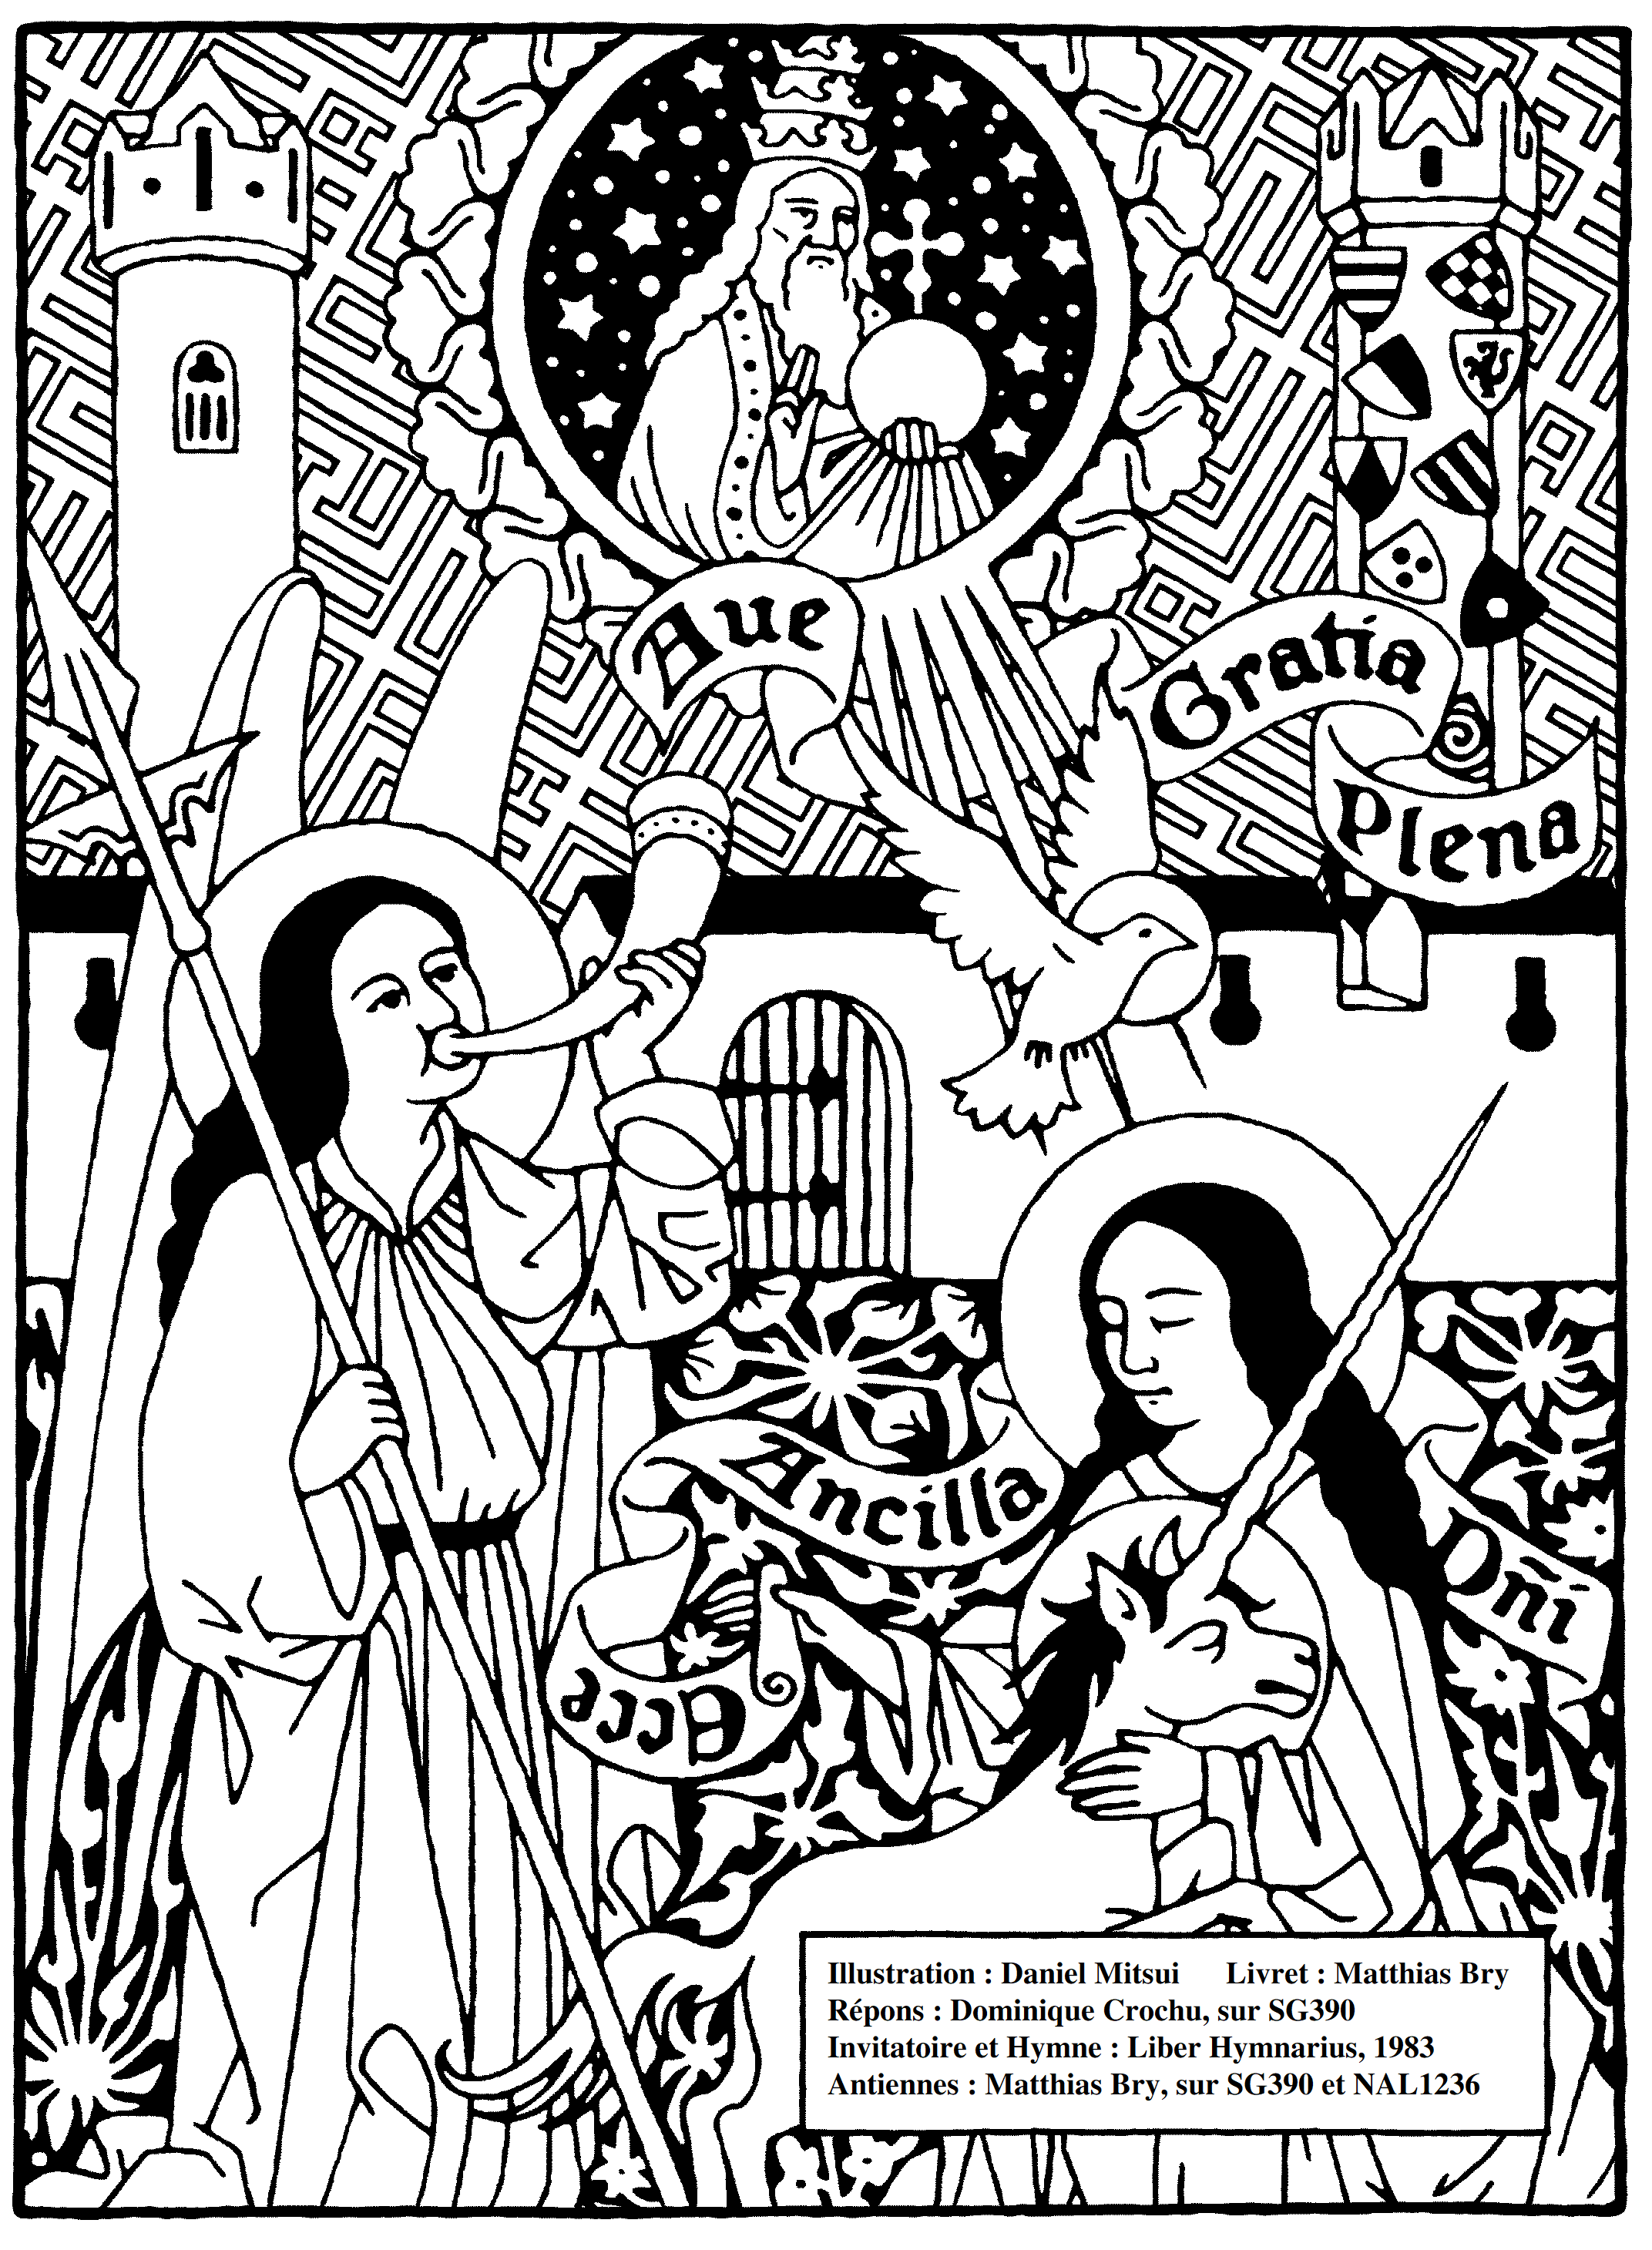
\includegraphics[width=13cm]{4ecouv.png}
\end{adjustwidth}
\end{document} 
